\documentclass[11pt]{article}

% ============================================================================
% Umbrella / review -- Transport, Not Computation. arXiv / Zenodo preprint.
% Compile: pdflatex x2.
% ============================================================================
\usepackage[utf8]{inputenc}
\usepackage[T1]{fontenc}
\usepackage{amsmath,amssymb}
\usepackage{graphicx}
\usepackage{booktabs}
\usepackage{geometry}
\usepackage{xcolor}
\usepackage[hidelinks]{hyperref}
\usepackage{caption}
\usepackage{enumitem}
\usepackage{authblk}

\geometry{a4paper, margin=1in}
\captionsetup{font=small, labelfont=bf}
\setlist{nosep, leftmargin=1.4em}

\title{\bfseries Transport, Not Computation:\\
A Cross-Model Falsification Program on How $1$B--$3$B Language Models\\
Use Long Context}

\author[1]{Evgenii Vyaltsev\thanks{ORCID 0009-0004-3712-6798. Correspondence: handle \texttt{@seqe\_phi}.}}
\author[1]{Daniil Vyaltsev}
\affil[1]{Independent Researcher}
\date{June 2026}

\begin{document}
\maketitle

\begin{abstract}
\noindent
We summarize a program of pre-registered, matched-control causal experiments on
small open language models (Llama-3.2-1B/3B, Qwen2.5-3B) that asks a single question:
when these models use long context, do they \emph{compute} internally or merely
\emph{transport} information? The program first establishes the substrate --- an exact,
training-free query-axis selector and the finding that long-context retention has
\emph{no critical key budget}: the sparse compressor is not the limit, the base model
is. It then runs four independent causal gates on the mechanism. \textbf{(1) Attention}
up-weighting a needed key is fully explained by plain re-delivery ($100\%\ge 80\%$):
attention is weighted transport. \textbf{(2) Delivery ladder:} the repair for
retrieval-disambiguation failure is delivering the attribute$\to$code binding ---
content-addressable, no positional decay, compressing to $27$ bytes --- while
attention-redirection and transplanted state-correction are both closed; a consistent
correction direction (skill score $0.46$ at L8) does \emph{not} transfer.
\textbf{(3) Synthesis} of an \emph{absent} multi-hop target reduces to
retrieval-and-elimination: corrupting the middle hop flips correct implicit answers in
only $5$--$11\%$ of cases (vs.\ $84$--$90\%$ for written chain-of-thought, the positive
control), and blocking elimination floors implicit accuracy to chance; genuine
traversal appears only as written, self-delivered CoT. \textbf{(4) Latent scratchpad:}
directly \emph{optimizing} a compact latent state (frozen weights) to switch failed
chains into composition yields only answer-injection on every control --- it carries
the target with the code fact removed, leaves intermediates lens-invisible, is inert to
hop corruption, and does not transfer --- closing the door that observation alone left
open. The four gates converge, cross-model and cross-family, on one thesis: \emph{in
this model class the network delivers, and composes only through an external buffer; it
does not latently compute, and a latent computation state cannot be optimized into
existence.} We argue the honest contribution is threefold: a map of the boundary of
internal competence (a chain of well-controlled NULLs, not a new ``intelligence''
mechanism); a constructive, training-free engineering result (an exact long-context
selector with an INT8 KV cache at $0.508\times$ footprint, plus a $27$-byte
micro-hint memory architecture); and a methodology (pre-registered matched-magnitude
controls that, en route, reversed two of our own false positives). All findings are
regime-bounded ($1$B--$3$B, retrieval and synthetic synthesis, greedy, $N\le128$K) and
do not transfer up the scale; each is released as a standalone artifact with raw logs.
\end{abstract}

\section{Introduction}
\label{sec:intro}

Does a language model \emph{think} over its context, or does it \emph{move} pieces of
it to the output? The distinction is mechanistic, not philosophical: a \emph{computing}
model forms new facts internally (binds $A,B,C$ into an absent $D$ at the answer step);
a \emph{transporting} model selects, delivers, and re-reads facts that are already
present, and composes --- when it composes at all --- by writing intermediate results
back into its own context. The two are behaviourally similar on easy tasks and
diverge exactly where it matters: long contexts, competition, and multi-step answers.

This paper is an umbrella over a program that pursued that distinction with one tool ---
the pre-registered, matched-magnitude causal gate --- across small open models. The
program's structure is deliberate. We first remove a confound: \emph{is the sparse
compressor itself the long-context bottleneck?} (No --- \S\ref{sec:engine}.) With the
compressor cleared, we ask, on the same models, \emph{where does competence actually
live}, through four gates that each pull a lever a system designer might reach for
(\S\ref{sec:gates}). The gates converge (\S\ref{sec:thesis}). We then state plainly what
the program is and is not (\S\ref{sec:map}), read off the engineering and product
consequences (\S\ref{sec:product}), and describe the methodology that makes the NULLs
trustworthy, including the false positives it caught and reversed (\S\ref{sec:method}).

\paragraph{Thesis.} Across Llama-3.2-1B/3B and Qwen2.5-3B, four independent causal
gates agree (Fig.~\ref{fig:arc}): \emph{the network delivers, and composes only through
an external buffer; it does not latently compute.} The result is regime-bounded and is
offered as a map of a boundary, not a universal law.

\begin{figure}[t]
\centering
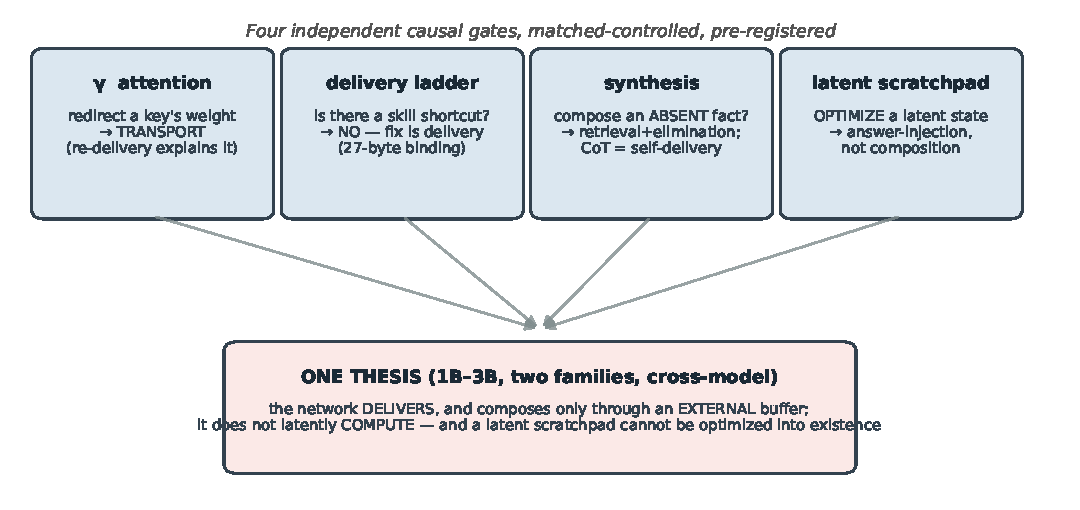
\includegraphics[width=0.96\textwidth]{figures/fig1_arc.pdf}
\caption{The program arc. Four independent, pre-registered, matched-control causal
gates --- on attention, on the repair of retrieval failure, on multi-hop synthesis,
and on a directly-optimized latent state --- converge on a single thesis, cross-model
and cross-family.}
\label{fig:arc}
\end{figure}

\section{The substrate: the compressor is not the limit}
\label{sec:engine}

Before asking how a model uses long context, we remove the obvious confound that a
\emph{sparse} engine might itself be the limiting factor.

\paragraph{An exact, training-free selector.} Ranking keys by the projection onto the
unit query direction $\mathbf{u}_Q=Q/\lVert Q\rVert$ is order-identical to ranking by
the raw attention score, so top-$k$ selection by $\langle\mathbf{u}_Q,K_i\rangle$
returns the \emph{true} top-$k$ with no learned parameters and no
approximation~\cite{paper2qaxis}. The cost of truncating to $k$ keys is governed by an
attention entropy that grows logarithmically, $H_N=\alpha\log N+\beta$ with measured
$\alpha\approx0.31$, so the effective support is sublinear ($N^{\alpha}$) and the
perplexity gap decays as $N^{-(1-\alpha)}$ --- the sparsity advantage \emph{strengthens}
with context (a descriptive scaling law; its causal status is held open).

\paragraph{No critical key budget.} Retrieval under semantic competition has \emph{no}
absolute key budget below which it collapses: holding the budget at fixed absolute
values and sweeping context length, a $4\times$ swing of the budget moves accuracy by
$\le0.03$ at any length, on three models~\cite{paper3retention}. The same budget holds
at $32$K yet fails at $65$K; the limit is the base model's own length-driven
disambiguation, not the compressor. Capacity \emph{raises the ceiling} (the
selected-yet-wrong fraction at $32$K falls $0.37\!\to\!0.23\!\to\!0.18$ from $1$B to
$3$B), and an INT8 KV cache realizes the engine at $0.508\times$ footprint for
$+0.714\%$ perplexity. With the compressor cleared as the bottleneck, the mechanism
question is well-posed: \emph{the limit is in the weights --- so what do the weights do
with the context?}

\section{Four causal gates}
\label{sec:gates}

Each gate is pre-registered, matched-controlled, and reported with the discipline of
\S\ref{sec:method}. Table~\ref{tab:gates} and Fig.~\ref{fig:sig} summarize; the
decisive numbers are recomputed from raw logs in each constituent paper.

\begin{table}[t]
\centering\small
\caption{The four gates. Each tests a lever; each verdict is delivery/transport.}
\label{tab:gates}
\begin{tabular}{p{2.5cm}p{4.2cm}p{6.4cm}}
\toprule
gate & decisive test & verdict \\
\midrule
$\gamma$ attention~\cite{paper3retention} & re-deliver the fact vs.\ up-weight its attention & \textbf{transport}: re-delivery ($100\%$) explains the weight effect ($80\%$); the attention-redirection class is closed \\
delivery ladder~\cite{paper4arc} & shrink the delivered payload; transplant a learned state correction & \textbf{delivery}: a $27$-byte binding recovers $100\%$ (content-addressable, no decay); bare code $58\%$; transplanted state ties random controls (not reusable) \\
synthesis~\cite{paper5synth} & corrupt each hop of an $A\!\to\!B\!\to\!C\!\to\!D$ chain; block elimination with decoys & \textbf{retrieval+elimination}: implicit mid-hop corruption flips $5$/$11\%$ vs.\ $84$/$90\%$ for CoT; implicit floors to chance under decoys; CoT traverses only by self-delivery \\
latent scratchpad~\cite{paper6latent} & optimize a latent state (frozen weights) to force composition; 5 controls & \textbf{answer-injection}: carries $D$ with the code fact removed ($0.94$/$0.81$), intermediates stay lens-invisible, inert to hop corruption, does not transfer --- no latent composition mode \\
\bottomrule
\end{tabular}
\end{table}

\begin{figure}[t]
\centering
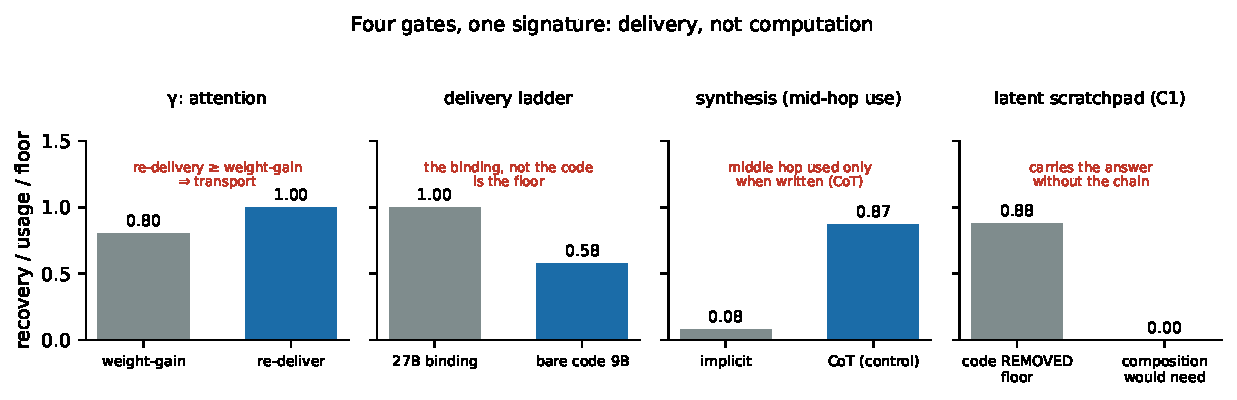
\includegraphics[width=\textwidth]{figures/fig2_signature.pdf}
\caption{Four gates, one signature. In each, the contrast that would distinguish
internal computation lands on the side of delivery/transport: re-delivery explains the
attention effect; the binding (not the bare code) is the floor; the middle hop is used
only when written down (CoT); and an optimized latent state carries the answer even
with the chain's content removed.}
\label{fig:sig}
\end{figure}

\paragraph{$\gamma$ --- attention is weighted transport.} On failure cases where the
needed key is selected yet the answer is wrong, multiplying its attention logits shifts
the answer strongly and needle-specifically ($\Delta P=+0.67$; a matched competitor
boost gives $-0.011$). But plain re-delivery of the same fact recovers at least as much
($100\%\ge80\%$): by the pre-registered rule the weight effect is fully explained by
delivery. Attention here moves information; it does not compute with it.

\paragraph{Delivery ladder --- the repair is a $27$-byte binding.} Re-delivering the
fact recovers $100\%$ at every distance up to $4096$ tokens (content-addressable, no
positional decay) and compresses losslessly to a $27$-byte attribute$\to$code binding;
stripping the binding to the bare code collapses recovery to $58\%$. Meanwhile a
learned hidden-state correction --- structured enough that its cross-case consistency
peaks sharply at one layer (skill score $0.46$) --- transplants to held-out cases no
better than random controls. The repair is neither attention redirection nor stored
weight-correction; it is delivery of the association.

\paragraph{Synthesis --- ``reasoning'' is retrieval-and-elimination.} Synthesis is the
adversarial case: the target $D$ is absent and must be assembled, so a pure transporter
should fail. It does not. Implicit (no scratchpad), corrupting the middle hop flips
correct answers in $5\%$/$11\%$ of cases while corrupting the code fact flips $100\%$;
masking the link facts at the answer step is inert; and adding decoys that block the
elimination shortcut floors implicit accuracy to chance ($0.35\!\to\!0.07$). The same
corruption machinery detects hop usage under chain-of-thought ($84$/$90\%$) --- the
built-in positive control proving the implicit null is real. CoT traverses genuinely,
but by writing each hop into context and re-reading it (self-delivery), not by internal
binding.

\paragraph{Latent scratchpad --- composition cannot be optimized into existence.}
Observation has a loophole: ``we did not see latent composition'' is weaker than ``there
is none''. So we search by optimization. With weights frozen, we gradient-optimize a
compact latent state to make failed chains emit $D$; five controls separate a
composition mode from a memorized answer. The optimizer succeeds at emitting $D$
(a single virtual vector suffices) but on every control it is answer-injection: it
carries $D$ with the code fact deleted ($0.94$/$0.81$), the intermediates never rise
from zero, hop corruption is inert, and it does not transfer; a CoT-informed
initialization does not rescue it. Even handed maximal freedom, the reachable solution
is delivery, not computation.

\section{One thesis}
\label{sec:thesis}

Four levers, four independent operationalizations, two architecture families, $1$B--$3$B:
the network selects and delivers facts, composes only when it can externalize the steps
into its own context, and shows no internal, decode-time formation of an absent fact ---
nor can such a state be optimized into being. \emph{Transport, not computation}, within
this regime. The synthesis and latent-scratchpad gates are the strongest legs precisely
because they are where transport \emph{should} have broken (an absent target; a free
optimizer aimed straight at composition) and did not.

This aligns with, and sharpens, several external observations: that attention heads move
information~\cite{elhage2021mathematical}; that latent multi-hop reasoning is weak and
training-dependent~\cite{yang2024latent,wang2024grokking}; that chain-of-thought traces
are not always faithful to an internal computation~\cite{lanham2023faithfulness}; and
that answers can be reached by elimination over the option
set~\cite{balepur2024elimination}. Our contribution is the causal, matched-control form
of these readings on off-the-shelf small models, and the constructive corollary that
follows.

\section{What the program is, and is not}
\label{sec:map}

\paragraph{What survived (the positives).} An \emph{exact, training-free long-context
selector} with a descriptive concentration scaling law and an INT8 KV cache; the finding
that \emph{retention is robust} and budget-insensitive up to where the base model itself
fails; a \emph{content-addressable delivery} result with a $27$-byte micro-hint floor; and
the demonstration that \emph{capacity, not key budget}, raises the long-context ceiling.

\paragraph{What was closed (the NULLs).} A spectral causal mechanism; an absolute
critical key budget; the attention-redirection class of memory schemes; transplanted
state-correction / skill-library; internal multi-hop composition at $3$B; and an
optimizable latent composition state. Each is a clean, controlled negative.

\paragraph{What is open.} Whether internal composition appears \emph{above} $3$B or with
trained chains; the exact channel of the above-chance implicit signal
(structural/positional/elimination); and a delocalization probe (does an answer survive
physical removal of the needed fact). None is closed here and none is claimed.

\paragraph{An honest framing.} We set out hoping to find an internal mechanism of
``intelligence'' and instead mapped, with triple controls, the boundary of internal
competence: in this regime it is delivery and externalized composition. That is the
honest result --- a boundary, not a breakthrough --- and it is more useful than a
narrative would have been. We resist the temptation to universalize: every gate is
$1$B--$3$B and regime-bounded, and a NULL at this scale does not transfer up.

\section{Engineering and product corollary}
\label{sec:product}

The program yields a concrete, training-free architecture for a local long-context
assistant, with each component justified by a gate rather than a hope:
\begin{itemize}
\item \textbf{Engine:} the exact query-axis selector plus the INT8 KV cache
($0.508\times$ footprint) --- longer context and lower memory on consumer hardware at
iso-ability. Sparsity buys speed and length, not intelligence; the safe operating
coverage is well above the recency floor.
\item \textbf{Memory:} store \emph{attribute$\to$code bindings} ($\sim$27 bytes),
retrieve by attribute, deliver freshly --- a RAG of micro-hints, content-addressable.
No attention-steering machinery and no skill-library adapter is warranted (both closed).
\item \textbf{Composition:} externalize it. Prompt the model to write its steps (CoT)
or run an explicit retrieve-compose loop (self-RAG); do not expect an internal chain or
a learned ``thinking'' vector to compose --- such a vector memorizes the answer.
\item \textbf{``Smarter''} on a fixed model comes from capacity or from better
delivery/scaffolding, not from the sparsity budget or an internal shortcut.
\end{itemize}

\section{Methodology: why the NULLs are trustworthy}
\label{sec:method}

Every gate fixes its grid, thresholds, controls, and verdict map \emph{before}
execution; none is tunable after. The signature move is the \emph{matched-magnitude
control}: a candidate cause is compared against a control of equal perturbation
magnitude (or equal information payload), and a pre-registered null closes the
direction. Verdicts are paired (within-run, immune to run-to-run nondeterminism) with
bootstrap CIs, and a positive after a NULL streak is held to extra scrutiny --- the
discipline that matters most when one \emph{wants} a positive.

The discipline earned its keep by catching false results: a spectral mechanism that
looked causal until a matched-magnitude control reversed it; a state-transfer ``signal''
at $17\%$ on $n{=}12$ that vanished at $n{=}60$; a smoke test that patched the wrong
layer and produced a false zero. A separate methodological catch is independently
useful: under competition, node \emph{removal} is confounded by elimination (a removed
fact is recoverable from competitors), so the faithful usage test is in-place
\emph{corruption}, not removal --- a distinction that flips conclusions about which hops
a chain ``uses''. The matched-control protocol is released as a standalone
note~\cite{matchedcontrols2026}.

\section{Limitations}
\label{sec:limits}

\begin{itemize}
\item \textbf{Scale and regime.} All gates are $1$B--$3$B, greedy, on retrieval and
synthetic multi-hop tasks, $N\le128$K (synthesis $N{=}4096$). Every NULL is
``not at this scale on this design'', not ``never''; the thesis does not transfer up.
\item \textbf{Tasks.} Semantic retrieval-under-competition and synthetic
attribute$\to$person$\to$zone$\to$code chains; natural reasoning, planning, and code are
separate gates.
\item \textbf{The descriptive scaling exponent} $\alpha$ is single-model/corpus and its
causal status is held open; the full multi-seed PPL sweep is a separate artifact.
\item \textbf{Off-distribution interventions} (attention forcing, mask-at-answer, latent
optimization) are off-distribution by construction; degeneration was distinguished from
clean answer-death, and ``optimization always finds something'' was defused by controls,
not assumed away.
\end{itemize}

\section{Conclusion}
\label{sec:conc}

A program of pre-registered, matched-control causal gates, cross-model over two
families and $1$B--$3$B, converges on one regime-bounded thesis: these models
\emph{transport} information and compose only through an external buffer; they do not
latently compute, and a latent computation state cannot be optimized into existence.
The honest yield is a map of the boundary of internal competence, a training-free
long-context engine and a $27$-byte micro-hint memory architecture justified by that
map, and a falsification methodology that reversed its own false positives. Whether
internal composition lives above this scale is the next program, and it should be
approached with the same matched-control skepticism that produced these results.

\section*{Program artifacts}
Each finding is a standalone release with raw logs, pre-registration, and a figure
script that recomputes its numbers. (1) Exact ranking + entropy scaling~\cite{paper2qaxis};
(2) No critical key budget~\cite{paper3retention} (DOI 10.5281/zenodo.20514229);
(3) The bottleneck is delivery~\cite{paper4arc};
(4) Even synthesis is transport~\cite{paper5synth};
(5) No latent scratchpad~\cite{paper6latent};
(6) Matched-magnitude controls~\cite{matchedcontrols2026} (DOI 10.5281/zenodo.20261207).
This umbrella references their verified headline numbers; the constituent repositories
hold the data and reproductions.

\begin{thebibliography}{99}
\small
\bibitem{paper2qaxis} E.\ Vyaltsev, D.\ Vyaltsev. \emph{Exact Query-Axis Ranking and Entropy-Concentration Scaling for Training-Free Top-K Sparse Attention}. Zenodo, 2026.
\bibitem{paper3retention} E.\ Vyaltsev, D.\ Vyaltsev. \emph{No Critical Key Budget in Query-Axis Top-K Sparse Attention}. Zenodo, DOI 10.5281/zenodo.20514229, 2026.
\bibitem{paper4arc} E.\ Vyaltsev, D.\ Vyaltsev. \emph{The Bottleneck Is Delivery}. Zenodo, 2026.
\bibitem{paper5synth} E.\ Vyaltsev, D.\ Vyaltsev. \emph{Even Synthesis Is Transport}. Zenodo, 2026.
\bibitem{paper6latent} E.\ Vyaltsev, D.\ Vyaltsev. \emph{No Latent Scratchpad}. Zenodo, 2026.
\bibitem{matchedcontrols2026} E.\ Vyaltsev, D.\ Vyaltsev. \emph{Matched-Magnitude Controls for Mechanistic Claims in Attention}. Zenodo, DOI 10.5281/zenodo.20261207, 2026.
\bibitem{elhage2021mathematical} N.\ Elhage et al. \emph{A Mathematical Framework for Transformer Circuits}. Anthropic, 2021.
\bibitem{yang2024latent} S.\ Yang et al. \emph{Do Large Language Models Latently Perform Multi-Hop Reasoning?} ACL, 2024.
\bibitem{wang2024grokking} B.\ Wang et al. \emph{Grokked Transformers are Implicit Reasoners}. NeurIPS, 2024.
\bibitem{lanham2023faithfulness} T.\ Lanham et al. \emph{Measuring Faithfulness in Chain-of-Thought Reasoning}. 2023.
\bibitem{balepur2024elimination} N.\ Balepur et al. \emph{Artifacts or Abduction: How Do LLMs Answer MCQs Without the Question?} ACL, 2024.
\end{thebibliography}

\end{document}
